\section{Program}
\label{section:program}

\begin{figure}[H]
  \centering
  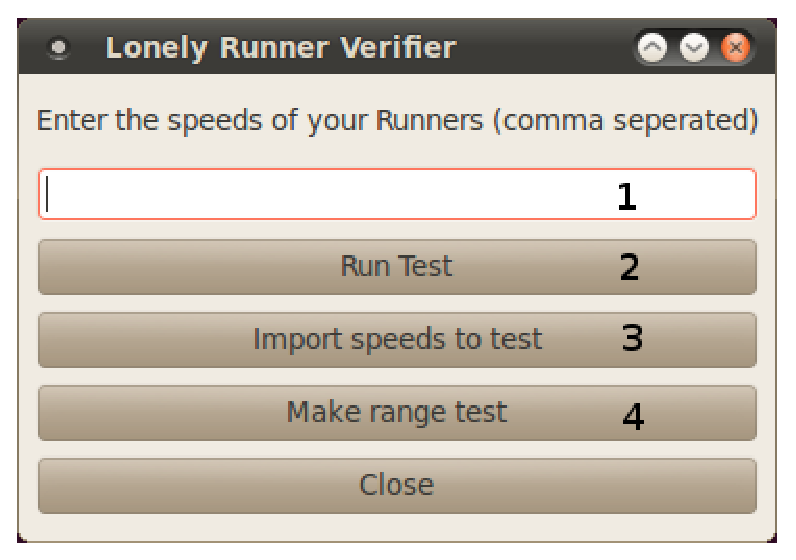
\includegraphics[width=0.45\textwidth]{./images/Lonely_Runner_Verifier}
  \caption{\label{fig:main_window}The main window of the program}
\end{figure}

The labels in figure \ref{fig:main_window} define the following:
\begin{enumerate}
\item The text field to manually enter runner speeds. The speeds must be in $\N$, and should be comma separated.
\item Run the test with the speeds entered in 1. Opens the option pane seen in figure \ref{fig:options}
\item Import the speeds from a JSON file (containing an array of integers). Opens the option pane seen in figure \ref{fig:options}
\item Test a range of configurations. Opens the option pane seen in figure \ref{fig:range_options}
\end{enumerate}

\begin{figure}[H]
  \centering
  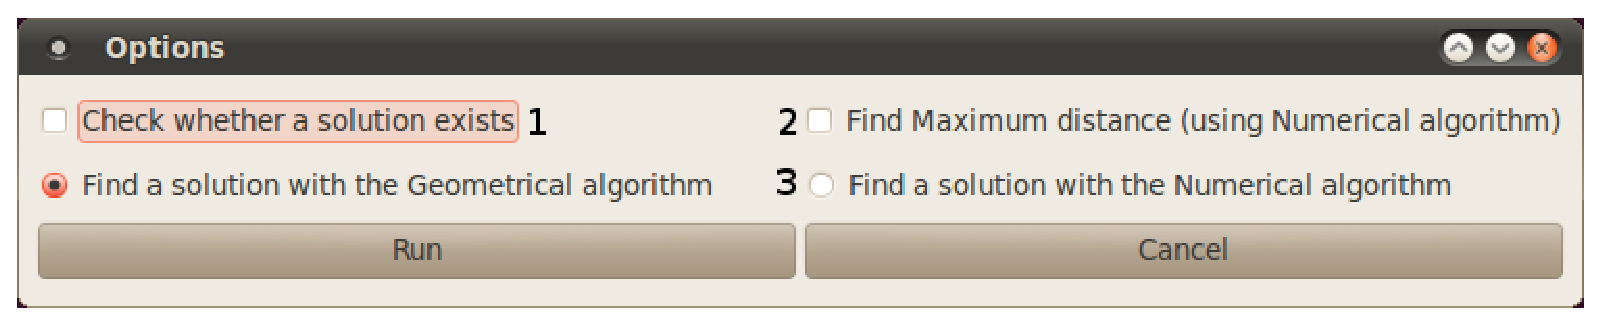
\includegraphics[width=0.70\textwidth]{./images/Options}
  \caption{\label{fig:options}The options for running a single configuration of runners. Accessed by either manually entering a speed or importing a runner configuration}
\end{figure}

The labels in figure \ref{fig:options} define the following:
\begin{enumerate}
\item If checked, the program will perform the check described in Section \ref{detect} before trying the algorithm selected in 3. This option is currently not compatible with option 2.
\item If checked, the program will find and report the maximum value that makes equation \eqaref{eqa:lonelyRunner} hold for the Numerical algorithm. Since this requires an exhaustive search, this can take a while\footnote{Since we in Section \ref{proof_num} established that the worst case run-time for the Numerical algorithm is $O(k * n^3)$, where $k$ is the sum of the 2 largest speeds, and $n$ is the number of Runners.} This option is not currently compatible with option 1.
\item Here you can define whether you would like the configuration to be checked with the Geometrical or the Numerical algorithm.
\end{enumerate}

\begin{figure}[H]
  \centering
  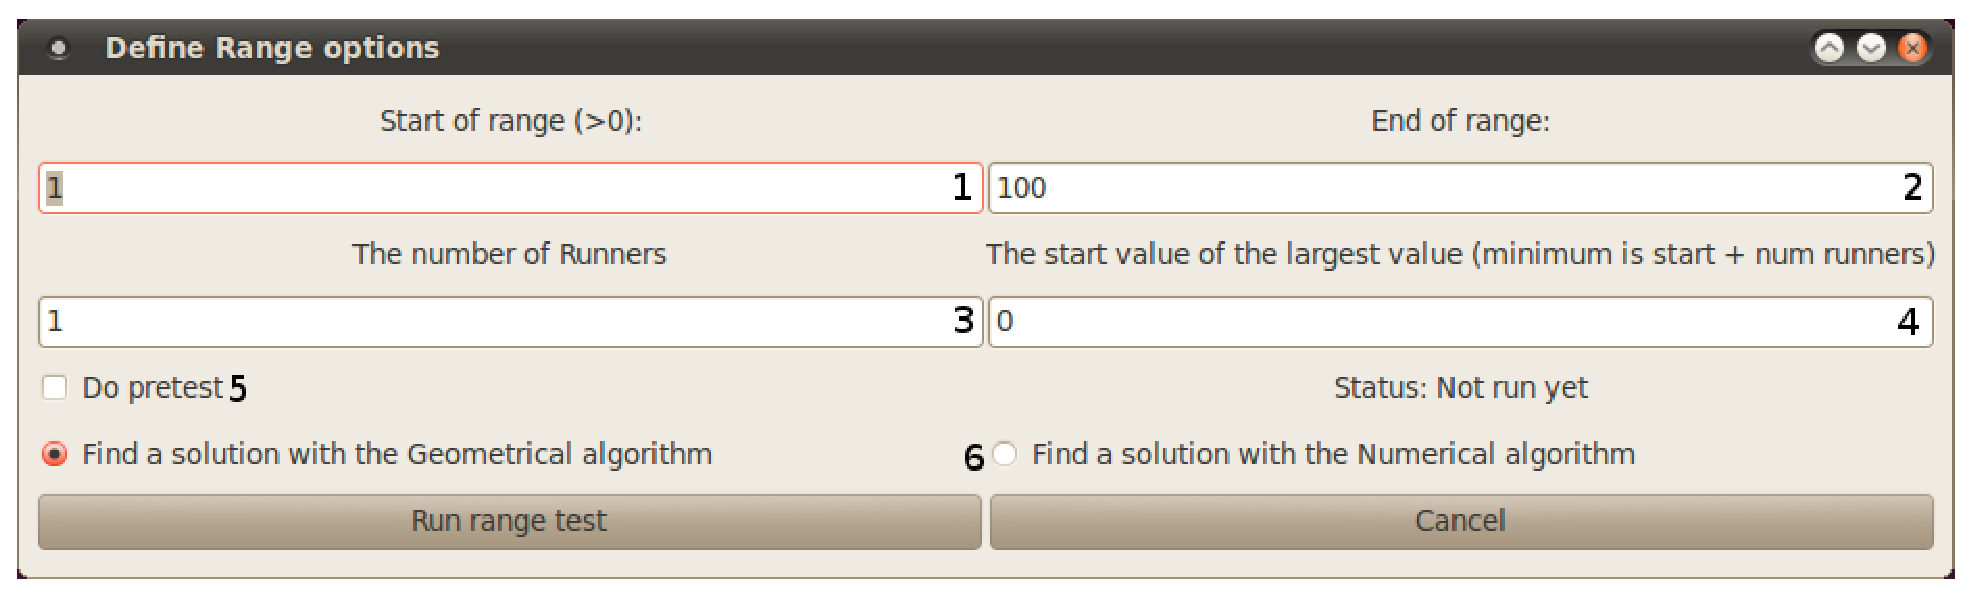
\includegraphics[width=0.70\textwidth]{./images/Range_Options}
  \caption{\label{fig:range_options}The options for running the Range Test}
\end{figure}

The labels in figure \ref{fig:range_options} define the following:
\begin{enumerate}
\item The minimum speed any runner can have 
\item The maximum speed any runner can have
\item The number of runners we are we are going to check
\item The start value of the largest speed. This option can be used as a primitive way to run the task in parallel on multiple computers, or can be used to resume the task at a certain speed. Let $d$ be the minimum speed plus the number of runners minus 1. If the value entered is less than $d$, then $d$ will be used instead.
\item The same as option 1 in figure \ref{fig:options}
\item The same as option 3 in figure \ref{fig:options}
\end{enumerate}

To give an example of the range test, let us say we wanted to test the range 1-10 with 3 runners.

Then the program would create and run the every possible configuration\footnote{This is done without regard to the order of the speeds, as it is clear this does not change the set of valid solutions to equation \eqaref{eqa:lonelyRunner}}, in this order:
$[1, 2, 3], [1, 2, 4], [1, 3, 4], [2, 3, 4], [1, 2, 5], \ldots, [1, 2, 10], \ldots, [7 ,9 ,10], [8, 9, 10]$.

If we still wanted to check the range 1-10 with 3 runners, but set the start value to 9, then the program would create and test the following combinations: 
$[1, 2, 9], [1, 3, 9], [2, 3, 9], \ldots, [7, 8, 9], [1, 2, 10], \ldots, [8, 9, 10]$

It should be clear from the examples above, that even for rather small numbers, a lot of test will be performed, so patience is advised. Since there are only a finite number of combinations, and every combination is either tested by the Geometrical or Numerical algorithm, both of which I have proved to terminate, then the Range Test must terminate.  
